\begin{wraptable}{r}{7.5 cm}
	\vspace{-10pt}
	
\begin{tabular}{|p{0.2\textwidth}|p{0.15\textwidth}|}
\hline
Tempo (secondi):&Numero di Nodi\\	
\hline
 0,859597206 & 1050 \\
0,839123964 & 1039 \\
0,812119007	& 1029 \\
0,807452917	& 1018 \\
0,782628059 & 1008 \\
0,764032125	& 997 \\
0,756317854 & 987 \\
0,732420921 & 976 \\
0,721984863	& 966 \\
0,719624996	& 955 \\
............................... & ........\\
0,0117771625518798 & 115 \\ 
0,00986480712890625 & 105 \\ 
0,00811696052551269 & 94 \\ 
0,00648427009582519 & 84 \\ 
0,00532007217407226 & 73 \\ 
0,00411915779113769 & 63 \\ 
0,00298309326171875 & 52 \\ 
0,00203299522399902 & 42 \\ 
0,00125527381896972 & 31 \\ 
0,00067305564880371 & 21 \\ 
0,000211000442504882 & 10 \\ 
\hline
\end{tabular}
\caption{Dati presentati in ordine discendente. (Il primo rappresenta la 100-esima iterazione mentre l'ultimo dato la prima) dell'esecuzione su grafi aciclici}\label{wrap-tab:1}
 % Really shortned Table
	\vspace{-10pt}
\end{wraptable} 
\section{Analisi Reale}
Per dare una "dimostrazione" di quanto detto prima, ovvero che il tempo dell'algoritmo sia un $O(|V|*|E|)$ ho pensato di realizzare un test, chiedendo al time di python di misurare 100 chiamate ( con elementi decrescenti ) ed osservarne il tempo di esecuzione.
\section{Alcuni Dati}
Nella tabella a fianco si possono osservare subito alcuni dati rilevanti scelti tra le prime e le ultime iterazioni. Ad ogni iterazione, per cercare di pesudo-randomizzare i dati alcune parti della funzioni \emph{generateCyclic/AcycleGraph} venivano modificate ad-hoc im tempo reale in relazione all'attuale i-esima iterazione. Tutti i dati raccolti durante le simulazioni  sono poi stati caricati in due fogli excel pronti per essere elaborati da Matlab per ottenere un grafico che possa mettere a confronto numero di nodi/tempo di esecuzione con il numero di nodi/$|V|*|E|$. Notevole di fatti è il dato del tempo di esecuzione ( espresso in secondi ) tranne in rare occasioni, da 1050 nodi a 10, si potrebbe dire che è rimasto "costante nel suo andamento simil-quadratico" rispetto alla quantità di nodi nell'input.
\section{Caratteristiche della Macchina:}I test sono stati effettuati su di un computer notte-tempo al fine di evitare qualsiasi interferenza da altri processi per l'accesso al disco o alle altre risorse del computer. La macchina su cui ho effettuato i test presenta le seguenti caratteristiche:
\begin{easylist}[itemize]
		& Produttore Apple -  Modello: 27"Mid2010
		& Processore: 2,8 GHz Intel Core i5
		& Memoria: 32 GB  DDR3  1333MHz - Disco: SSD Samsung 500 GB
		& Sistema Operativo: OS X El Capitain ( Versione: 10.11.6 (15G17023) )
\end{easylist}

\section{Andamenti a Confronto}
Attraverso Matlab, ho ottenuto i seguenti grafici che evidenziano ancora di più l'andamento temporale dell'algoritmo e del $|V|*|E|$.\\ \\
\begin{figure}[H]
\vspace{-10pt}
    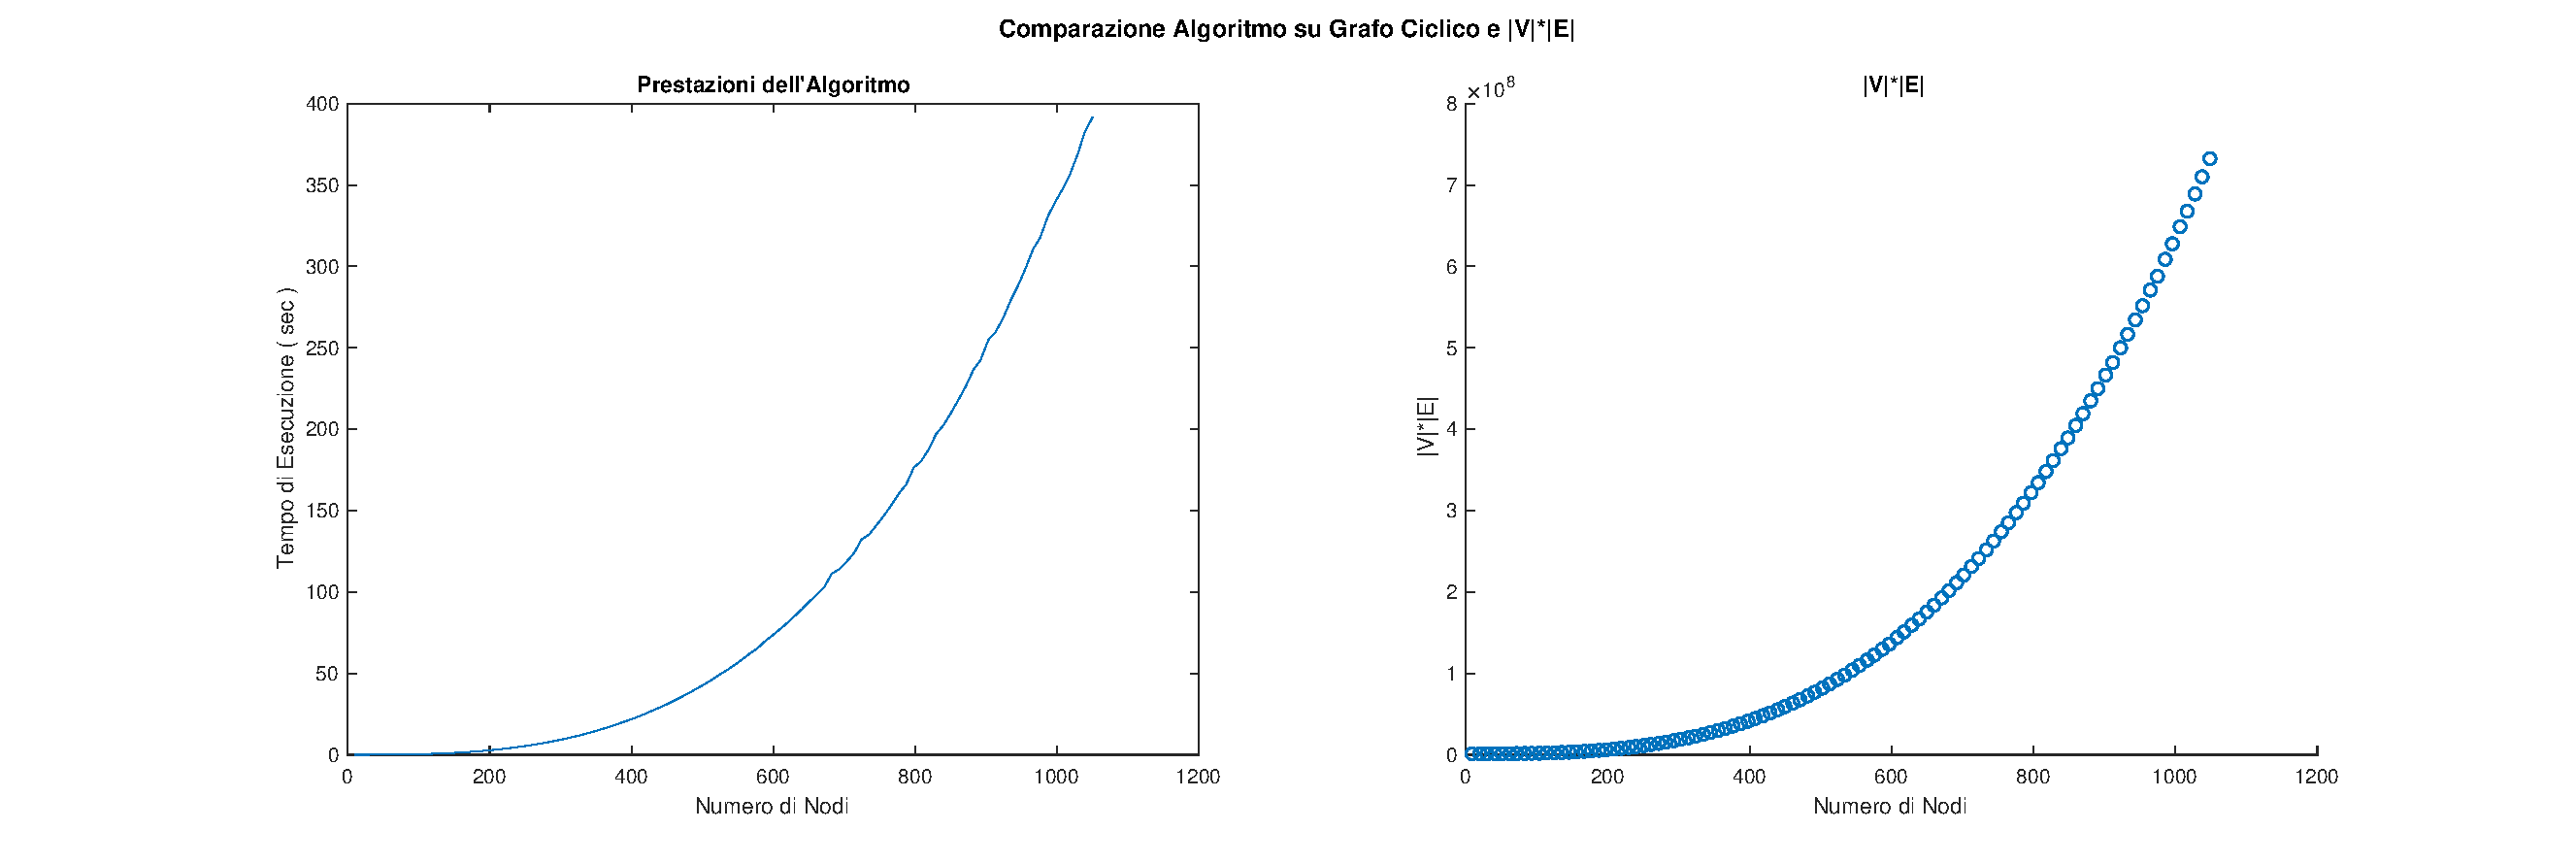
\includegraphics[width=\textwidth,height=\textheight,keepaspectratio]{./TeX_files/chart/Ciclico}
    \caption{Grafico che mette a confronto numero di nodi/tempo di esecuzione e  numero di nodi/$|V|*|E|$ per grafi Ciclici}
\vspace{-10pt}
\end{figure}

\begin{figure}[H]
	\vspace{-10pt}
	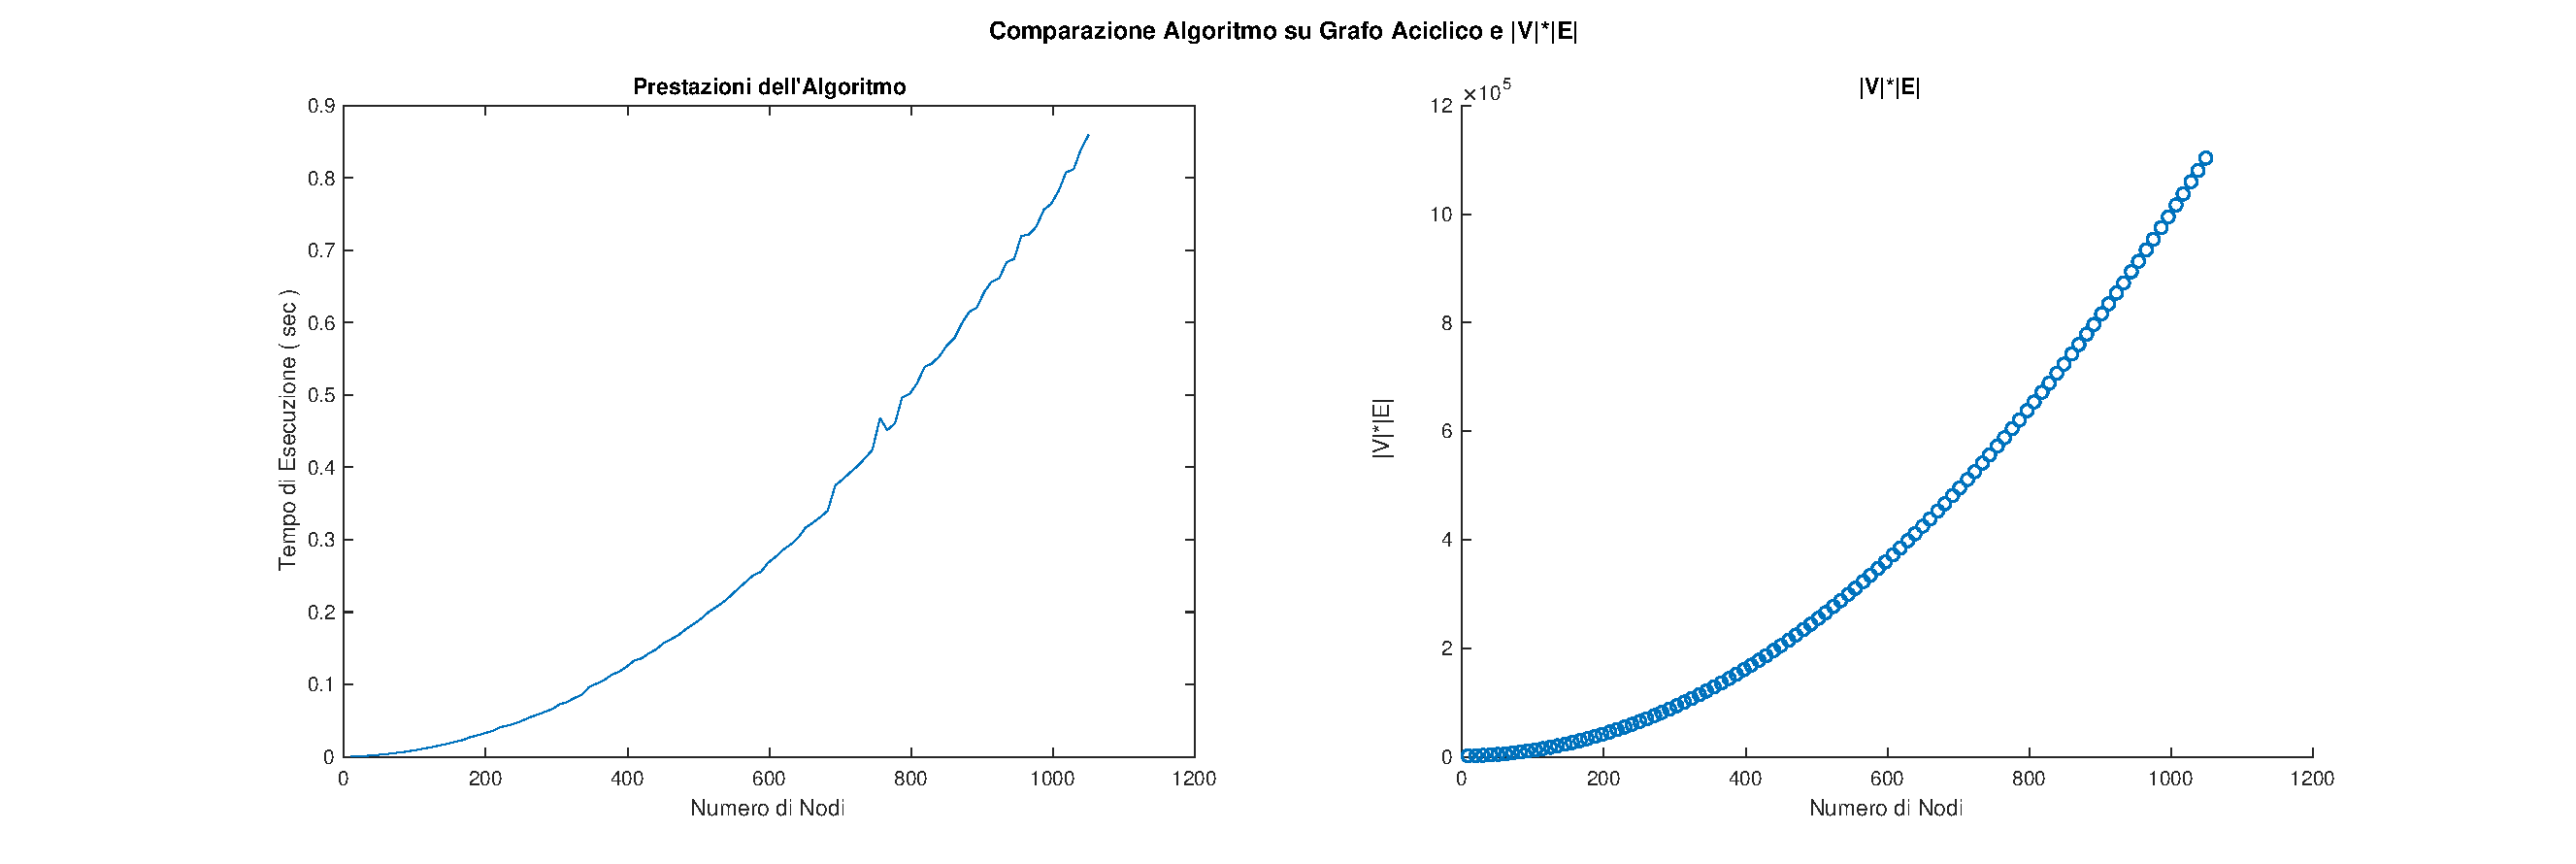
\includegraphics[width=\textwidth,height=\textheight,keepaspectratio]{./TeX_files/chart/Aciclico}
	\caption{Grafico che mette a confronto numero di nodi/tempo di esecuzione e  numero di nodi/$|V|*|E|$ per grafi Aciclici}
	\vspace{-10pt}
\end{figure}

\noindent Come si evince dalle Figure 4.1-2, la complessità temporale studiata teoricamente nell'analisi teorica dell'algoritmo è risultata corretta e supportata da evidenze sperimentali. Data una ricerca più approfondita in materia, l'algoritmo di Brandes detiene tutt'ora adesso il "primato" ( se pur nel recente periodo sia stato ampliato e ancora più raffinato ), pur essendo un algoritmo di carattere statico e avendo validissimi algoritmi di tipologia euristica come avversari. La peculiarità del presente algoritmo è insita nella "intrinseca parallelità". É infatti possibile modificare l'algoritmo e adattarlo ad una tipologia di approccio clusteristico nel quale si può demandare il calcolo dei cammini minimi e delle dipendenze a diversi core di elaborazione e quindi eseguire il tutto in parallelo.

